\documentclass[12pt, a4paper]{report}
\usepackage[utf8]{inputenc}
\usepackage[english, russian]{babel}

\usepackage{graphicx}
\usepackage{listings}
\usepackage{color}

\usepackage{amsmath}
\usepackage{pgfplots}
\usepackage{url}
\usepackage{flowchart}
\usepackage{tikz}
\DeclareGraphicsExtensions{.pdf,.png,.jpg,.svg}
\usetikzlibrary{shapes, arrows}

\usepackage{pgfplotstable}

\renewcommand\contentsname{Содержание}

\usepackage{geometry}
\geometry{left=3cm}
\geometry{right=1cm}
\geometry{top=2cm}
\geometry{bottom=2cm}

\lstset{ %
language=C++,                 % выбор языка для подсветки (здесь это С)
basicstyle=\small\sffamily, % размер и начертание шрифта для подсветки кода
numbers=left,               % где поставить нумерацию строк (слева\справа)
numberstyle=\tiny,           % размер шрифта для номеров строк
stepnumber=1,                   % размер шага между двумя номерами строк
numbersep=-5pt,                % как далеко отстоят номера строк от         подсвечиваемого кода
backgroundcolor=\color{white}, % цвет фона подсветки - используем         \usepackage{color}
showspaces=false,            % показывать или нет пробелы специальными     отступами
showstringspaces=false,      % показывать или нет пробелы в строках
showtabs=false,             % показывать или нет табуляцию в строках
frame=single,              % рисовать рамку вокруг кода
tabsize=2,                 % размер табуляции по умолчанию равен 2 пробелам
captionpos=t,              % позиция заголовка вверху [t] или внизу [b] 
breaklines=true,           % автоматически переносить строки (да\нет)
breakatwhitespace=false, % переносить строки только если есть пробел
escapeinside={\%*}{*)},   % если нужно добавить комментарии в коде
keywordstyle=\color{blue}\ttfamily,
stringstyle=\color{red}\ttfamily,
commentstyle=\color{green}\ttfamily,
morecomment=[l][\color{magenta}]{\#},
columns=fullflexible }

\usepackage{titlesec}
\titleformat{\chapter}[hang]{\LARGE\bfseries}{\thechapter{.} }{0pt}{\LARGE\bfseries}
\titleformat*{\section}{\Large\bfseries}
\titleformat*{\subsection}{\large\bfseries}

\begin{document}

    \begin{titlepage}

        \begin{center}
            \Large
            {\sl Государственное образовательное учреждение высшего профессионального образования\\
            {\bf«Московский государственный технический университет имени Н.Э. Баумана»\\
				(МГТУ им. Н.Э. Баумана)}}
            \vspace{3cm}

			{\scshape\LARGE Лабораторная работа №... \par}
			\vspace{0.5cm}	
			{\scshape\LARGE по курсу «Анализ алгоритмов» \par}
			\vspace{1.5cm}
			{\huge\bfseries Тема лабораторной работы \par}
			\vspace{2cm}
			\Large Выполнил: Тимонин А.С., гр. ИУ7-52Б\\
			\vspace{0.5cm}
			{\Large Преподаватели: Волкова Л.Л., Строганов Ю.В.}
		
			\vfill
			\Large \textit {2019 г.}
            
        \end{center}

    \end{titlepage}
	
	\tableofcontents

	\chapter*{Введение}
	\addcontentsline{toc}{chapter}{Введение}
	

    \chapter{Аналитический раздел}
   	\vspace{-0.5cm}бла-бла-бла
	\section{Описание алгоритмов}
	бла-бла-бла

	\section{Алгоритм1}
	
	\section{Алгоритм2}
	бла-бла-бла
	

	\chapter{Конструкторский раздел}
	
	\vspace{-0.5cm} bla-bla-bla
	
	\section{Разработка алгоритмов}
	тут схема алгоритмов

	\newpage

	\section{Расчет сложности}
	бла-бла-бла
	
	\section{Вывод}
	бла-бла-бла
	
	\begin{itemize}
		\item бла-бла-бла
		\item бла-бла-бла
		\item бла-бла-бла
	\end{itemize}
	
	\chapter{Технологический раздел}
	\vspace{-0.5cm}бла-бла-бла
	
	\section{Требования к программному обеспечению}
	бла-бла-бла
	\section{Средства реализации}
	\hspace{0.6cm}Для выполнения поставленной задачи был использован язык программирования С++. Среда для разработки XCode. Для измерения процессорного времени была взята функция rdtsc из библиотеки ctime.
	
	\vspace{0.2cm}Данный язык обусловлен тем, что функции замеры времени могут считывать не только абсолютное время, но и процессорное.
	
	\vspace{0.2cm}Версия компилятора C++: GNU++14 [-std=gnu++14]
	
	
	
	\section{Листинг кода}
	бла-бла-бла

	\begin{lstlisting}[label=code-opt,caption=бла-бла-бла]
	void name(int a)
	{
		return;
	}
	\end{lstlisting}

	\newpage

	\section{Вывод}
	бла-бла-бла

			
	\chapter{Экспериментальный раздел}
	
	\vspace{-0.6cm}\hspace{0.5cm}В данном разделе будет приведено экспериментальное исследование временных затрат разработанного программного обеспечения, вместе в подробным сравнительным анализом реализованных алгоритмов на основе экспериментальных данных.
	
	\section{Сравнительный анализ}
	
	\hspace{0.6cm}Замеры времени выполнялись на квадратных матрицах размеров от 100х100 до 1000х1000 с интервалом в 100 элементов. Также замеры времени проводились над квадратными матрицами нечетной размерностью  от 101х101 до 1001х1001 с шагом 100. В табл. \ref{table1}-\ref{table2} и рис. \ref{pic1}-\ref{pic2} представлены результаты замеров времени в тактах.
	
	\vspace{0.3cm}Замеры времени выполнялись на тестах...... Все замеры проводились на процессоре 1,4 GHz Intel Core i5 с памятью 8 ГБ 2133 MHz LPDDR3.
	
	\begin{table}[ht!]
		\caption{Сравнение времени работы однопоточной и многопоточной версий алгоритма в единицах измерения библиотеки chrono}
		\label{table1}
		\begin{center}
			\begin{tabular}{|c|c|c|c|c|}
				\hline
				\bf{Размерность матриц} & \bf{Поток 1} & \bf{Поток 2} & \bf{Поток 4} & \bf{Поток 8}\\\hline
				
				$100$ & $4$ & $1$ & $1$ & $1$\\\hline
				
				$200$ & $29$ & $10$ & $7$ & $6$\\\hline
				
				$300$ & $134$ & $49$ & $25$ & $25$\\\hline
				
				$400$ & $365$ & $138$ & $102$ & $71$\\\hline
				
				$500$ & $743$ & $283$ & $185$ & $135$\\\hline
				
				$600$ & $1206$ & $450$ & $247$ & $210$\\\hline
				
				$700$ & $1886$ & $757$ & $435$ & $364$\\\hline
				
				$800$ & $3029$ & $1112$ & $782$ & $531$\\\hline
				
				$900$ & $7909$ & $2463$ & $1028$ & $860$\\\hline
				
				$1000$ & $12799$ & $3660$ & $2047$ & $1476$\\\hline
			\end{tabular}
		\end{center}
	\end{table}

	\newpage

	\begin{figure}[ht!]
		\label{pic1}
		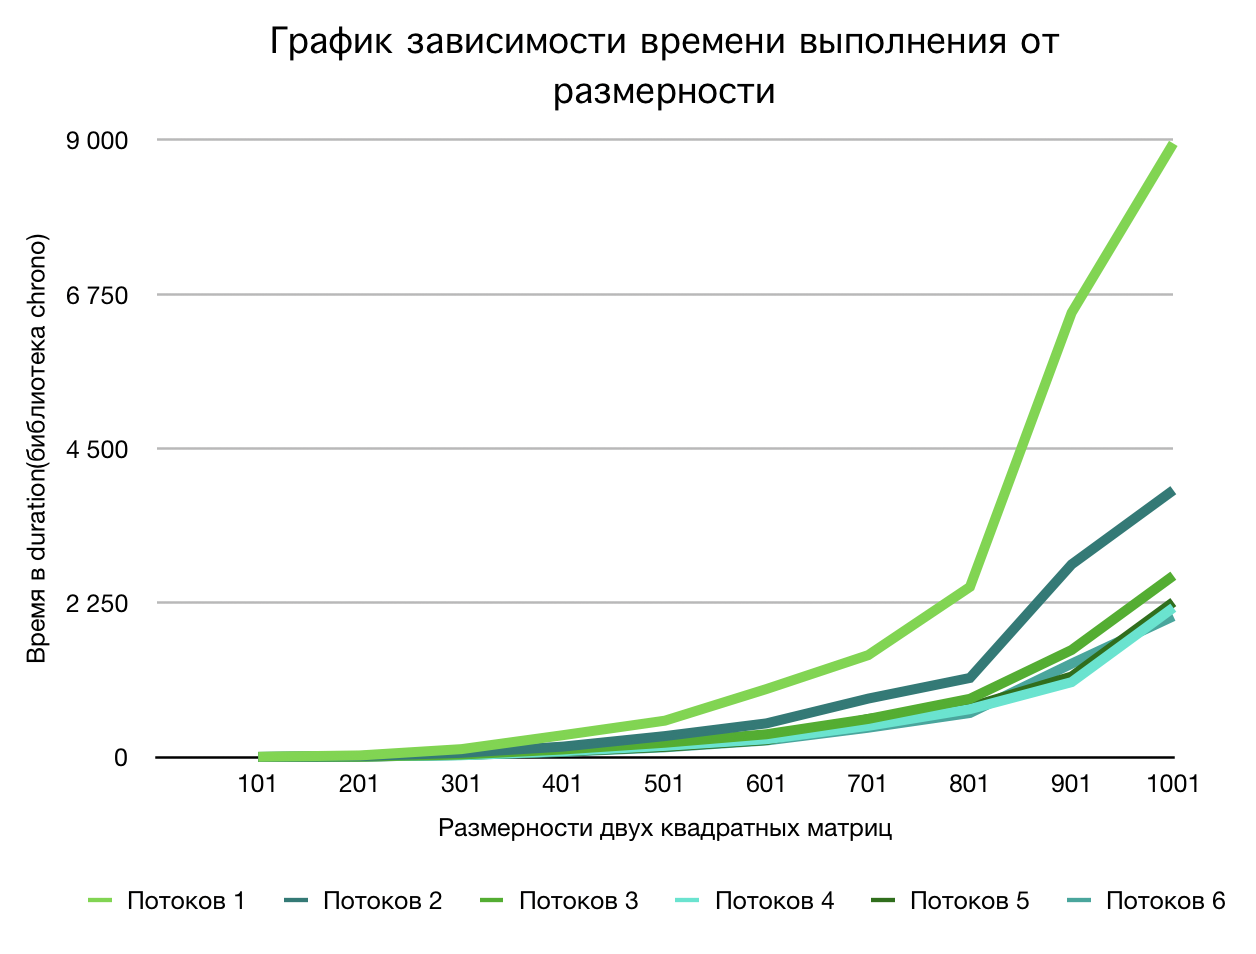
\includegraphics[scale=1.2]{table2}
		\caption{График зависимости времени работы однопоточной и многопоточных версий 	алгоритма для четной размерности матриц}
		\label{fig:image}
	\end{figure}

	\newpage

	\begin{table}[ht!]
		\caption{Сравнение времени работы однопоточной и многопоточной версий алгоритма 	в единицах измерения библиотеки chrono}
		\label{table2}
		\begin{center}
			\begin{tabular}{|c|c|c|c|c|}
				\hline
				\bf{Размерность матриц} & \bf{Поток 1} & \bf{Поток 2} & \bf{Поток 4} & \bf{Поток 	8}\\\hline
			
				$101$ & $4$ & $2$ & $1$ & $1$\\\hline
			
				$201$ & $30$ & $11$ & $5$ & $6$\\\hline
			
				$301$ & $120$ & $51$ & $25$ & $25$\\\hline
			
				$401$ & $363$ & $135$ & $82$ & $65$\\\hline
			
				$501$ & $707$ & $267$ & $143$ & $128$\\\hline
			
				$601$ & $1202$ & $444$ & $236$ & $206$\\\hline
			
				$701$ & $1954$ & $782$ & $391$ & $346$\\\hline
			
				$801$ & $3161$ & $1174$ & $592$ & $640$\\\hline
			
				$901$ & $6120$ & $2502$ & $1305$ & $1204$\\\hline
			
				$1001$ & $9314$ & $3766$ & $2400$ & $2186$\\\hline
			\end{tabular}
		\end{center}
	\end{table}

	%\newpage
	
	\begin{figure}[ht!]
		\label{pic2}
		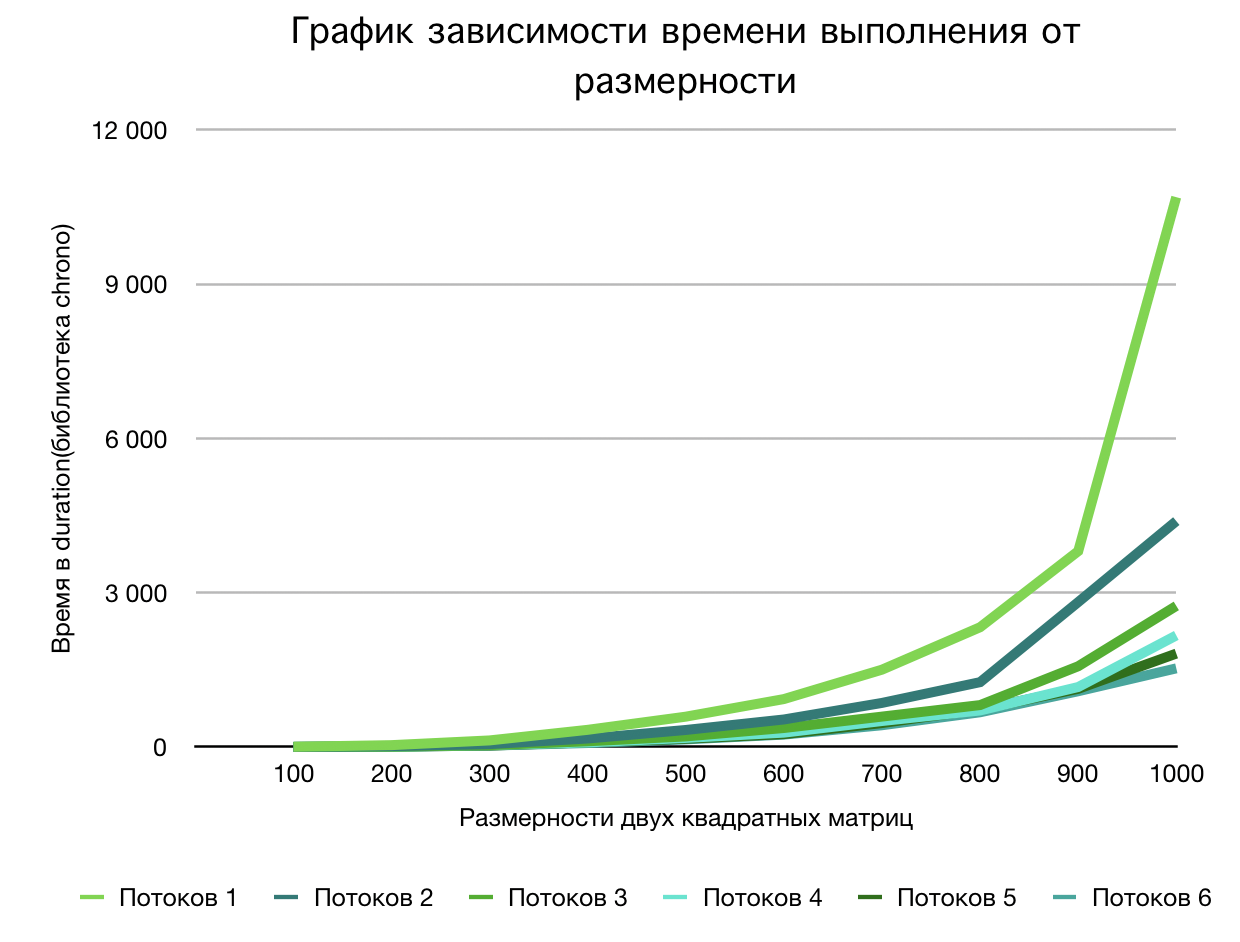
\includegraphics[scale=1.2]{table1}
		\caption{График зависимости времени работы однопоточной и многопоточных версий алгоритма для нечетной размерности матриц}
		\label{fig:image}
	\end{figure}

	Из данных графиков видно, что присутствие хотя бы двух потоков в несколько раз эффективнее, в сравнению с однопоточной реализацией алгоритма. Разница по времени выполнения в многопоточной реализации алгоритма не зависит от четной или нечетной размерности матриц. Самое опитмальное количество потоков для реализации данного алгоритма - 4, из-за того что на восьми потоках разниц не существенна. 
	\newpage
	
	\section{Вывод}
	
	\hspace{0.6cm}В данном разделе было проведено исследование однопоточной и многопоточных версий алгоритма. Приведены графики зависимостей времени работы алгоритма от размерности матриц.
	
	\vspace{0.3cm}Среди всех версий алгоритма самыми лучшим оказались версии, где задействовалось не менее четырех потоков. Многопоточная версия алгоритмов показала хороший реазультат относительно однопоточной версии: восьмипоточная реализация алгоритма эффективней однопоточной на 400\% при размерности матриц равной 1000.

	\newpage
	
 	бла-бла-бла

	\chapter*{Заключение}
	\addcontentsline{toc}{chapter}{Заключение}
	бла-бла-бла
	
	\newpage
	
	\begin{thebibliography}{}
	\bibitem ...
	\end{thebibliography}
	\addcontentsline{toc}{chapter}{Литература}

\end{document}